\subsection{Baum-Welch Convergence}
\label{fig:convergence}

Figure~\ref{fig:convergence_all} shows the Baum-Welch convergence curves for all five state resolutions.
All models converged within 60 iterations, with larger $K$ values requiring slightly more iterations to stabilize.

\begin{figure}[H]
\centering
\begin{subfigure}[b]{0.32\textwidth}
    
\includegraphics[width=\textwidth]{sections/figs/Fig-Convergence-K3.pdf}
    \caption{$K = 3$}
\end{subfigure}
\hfill
\begin{subfigure}[b]{0.32\textwidth}
    
\includegraphics[width=\textwidth]{sections/figs/Fig-Convergence-K9.pdf}
    \caption{$K = 9$}
\end{subfigure}
\hfill
\begin{subfigure}[b]{0.32\textwidth}
    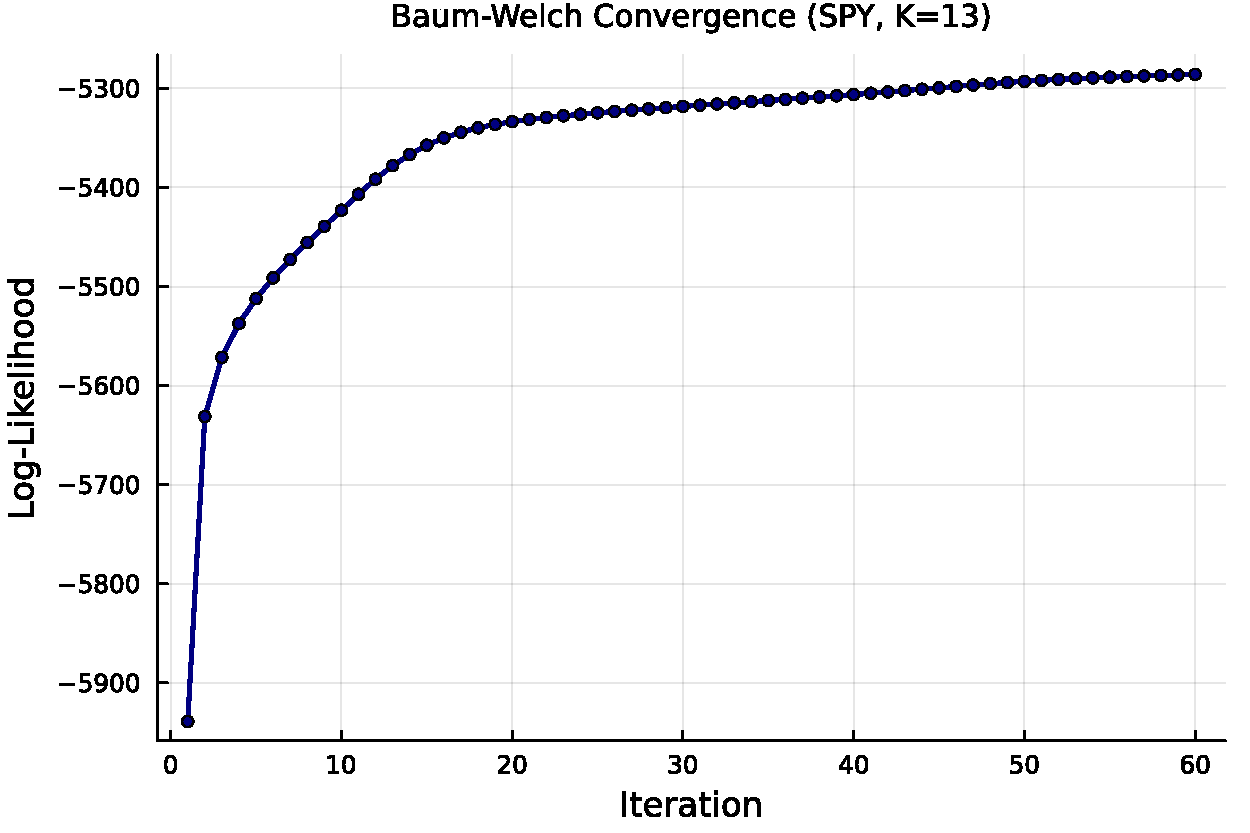
\includegraphics[width=\textwidth]{sections/figs/Fig-Convergence-K13.pdf}
    \caption{$K = 13$}
\end{subfigure}
\caption{Baum-Welch convergence for selected state resolutions. Log-likelihood is monotonically increasing (EM guarantee) and plateaus before \texttt{max\_iter} = 60.}
\label{fig:convergence_all}
\end{figure}

\subsection{Grid Search Landscapes}

Figure~\ref{fig:grid_search_all} shows the jump hyperparameter grid search landscapes for $K = 3$ and $K = 13$.

\begin{figure}[H]
\centering
\begin{subfigure}[b]{0.48\textwidth}
    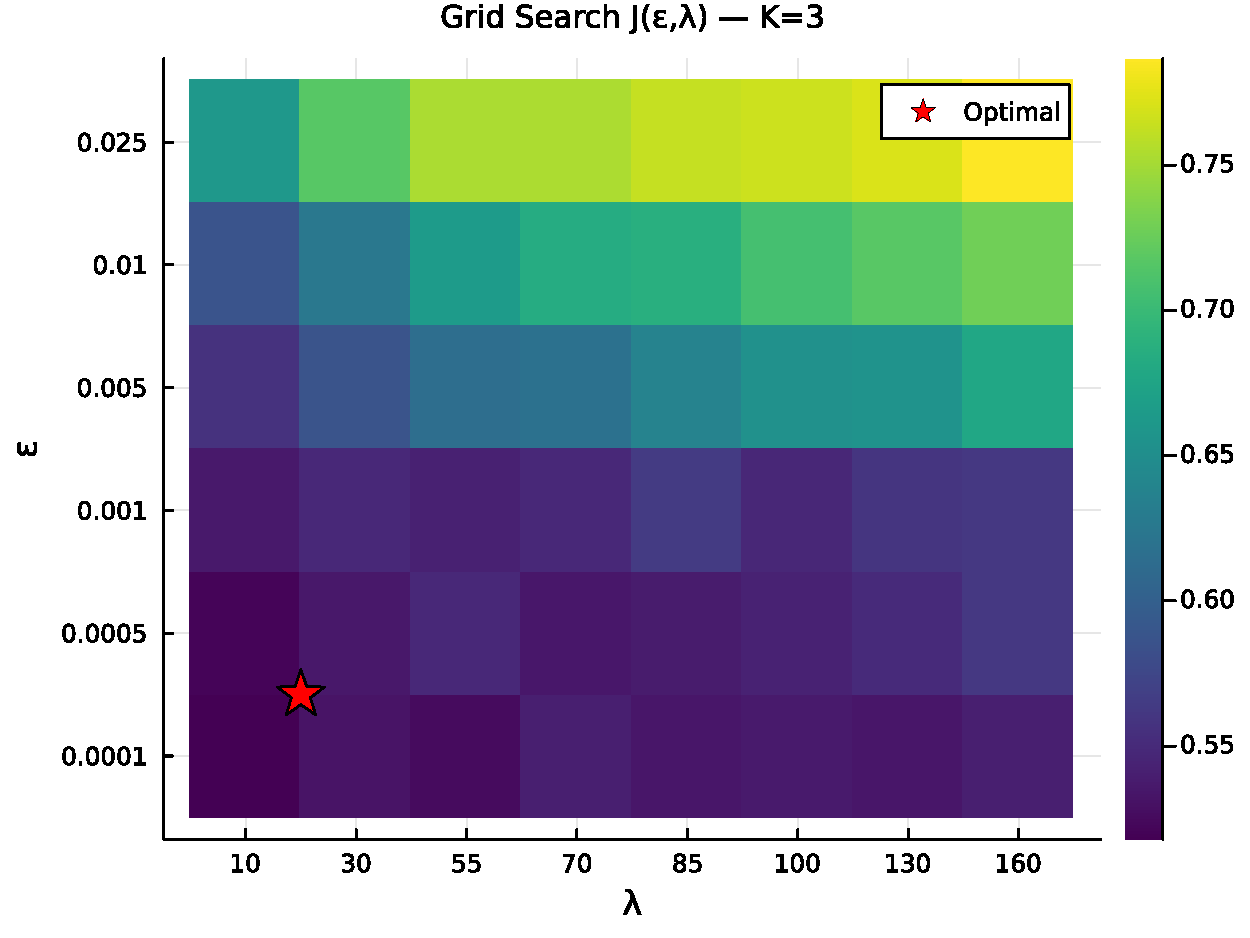
\includegraphics[width=\textwidth]{sections/figs/Fig-Grid-Search-K3.pdf}
    \caption{$K = 3$ ($\epsilon^* = 10^{-4}$, $\lambda^* = 10$)}
\end{subfigure}
\hfill
\begin{subfigure}[b]{0.48\textwidth}
    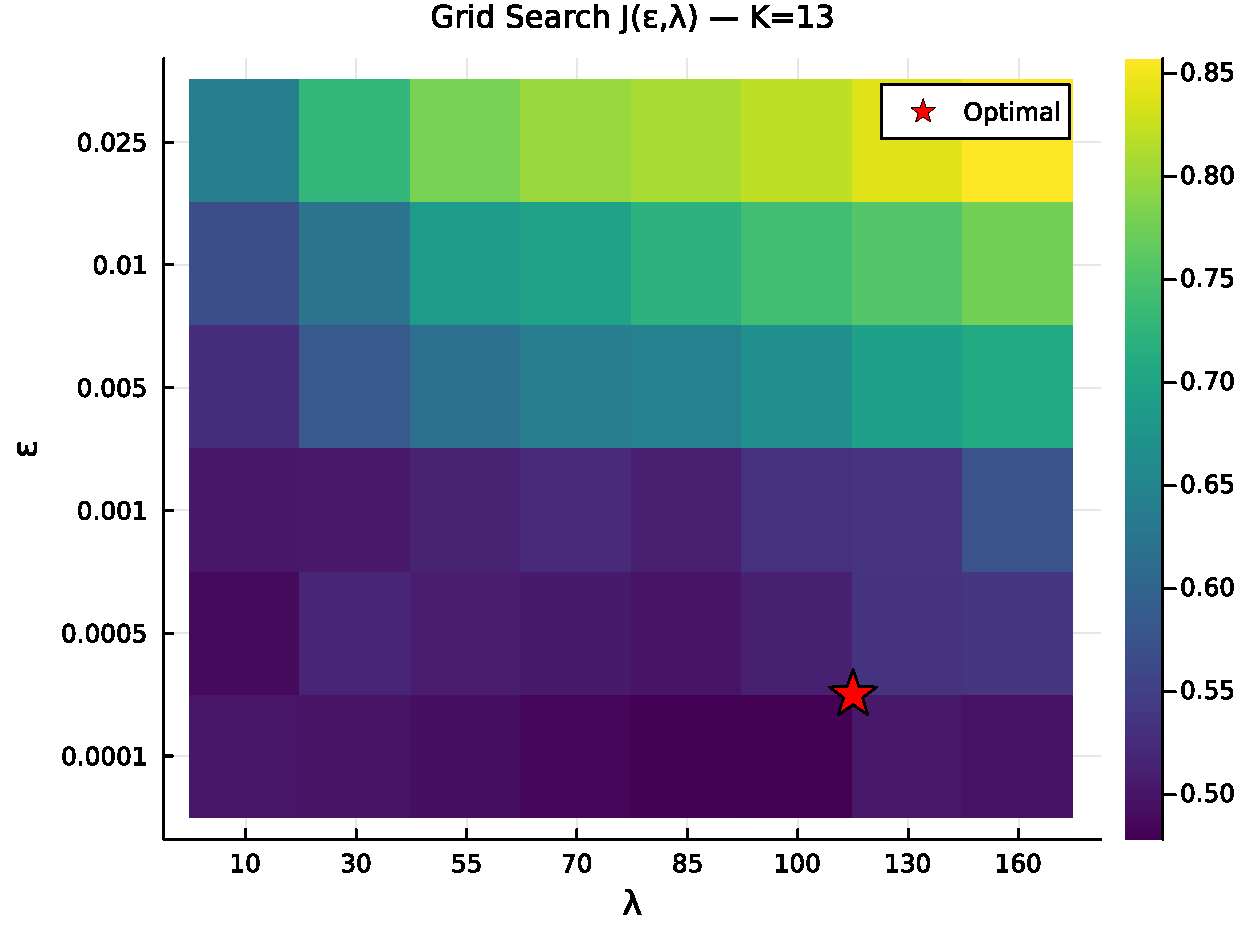
\includegraphics[width=\textwidth]{sections/figs/Fig-Grid-Search-K13.pdf}
    \caption{$K = 13$ ($\epsilon^* = 10^{-4}$, $\lambda^* = 100$)}
\end{subfigure}
\caption{Grid search heatmaps of the objective function $J(\epsilon, \lambda)$ in log$_{10}$ scale. Red stars mark the optimal parameters. The clear minima confirm that the jump hyperparameters are jointly identifiable from data.}
\label{fig:grid_search_all}
\end{figure}

\subsection{Emission Distributions Across State Resolutions}

Figure~\ref{fig:emissions_all} compares the learned emission structures for $K = 3$, $K = 9$, and $K = 13$.

\begin{figure}[H]
\centering
\begin{subfigure}[b]{0.32\textwidth}
    
\includegraphics[width=\textwidth]{sections/figs/Fig-Emission-PDFs-K3.pdf}
    \caption{$K = 3$}
\end{subfigure}
\hfill
\begin{subfigure}[b]{0.32\textwidth}
    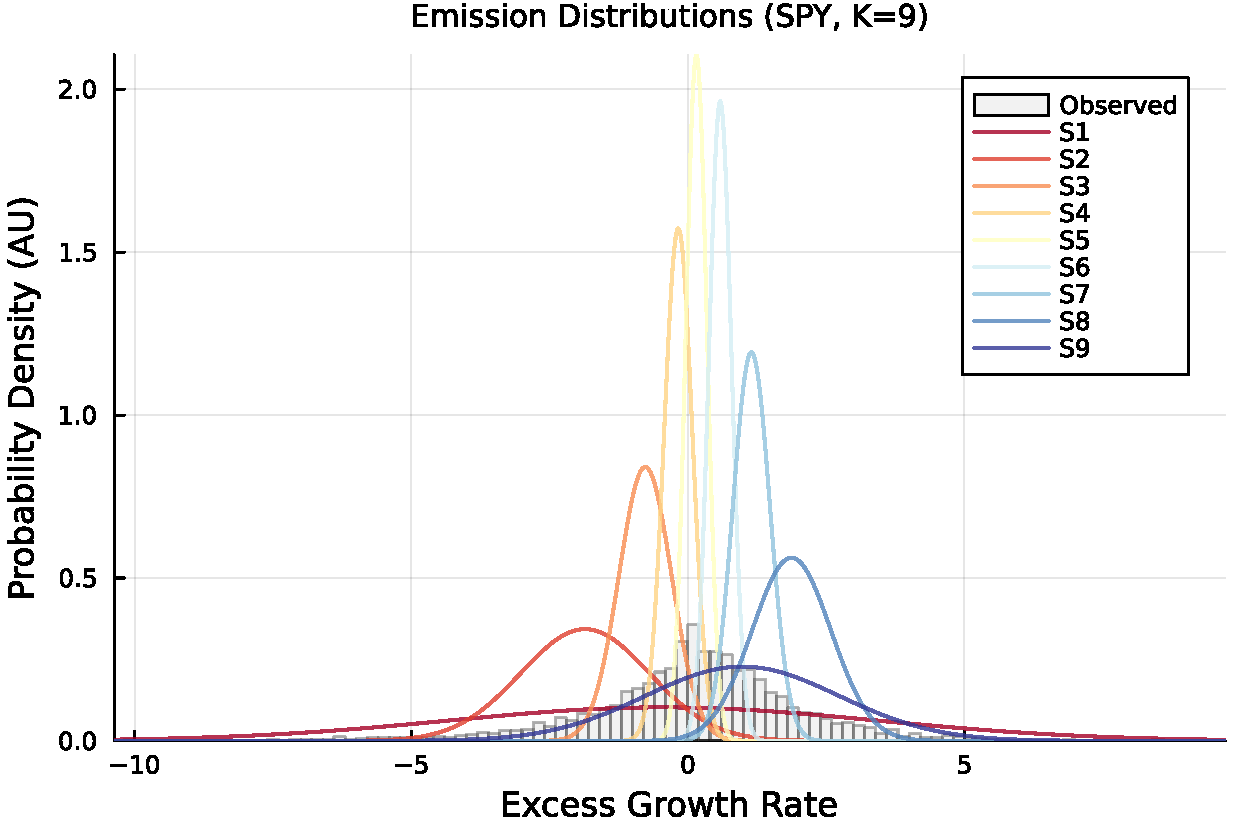
\includegraphics[width=\textwidth]{sections/figs/Fig-Emission-PDFs-K9.pdf}
    \caption{$K = 9$}
\end{subfigure}
\hfill
\begin{subfigure}[b]{0.32\textwidth}
    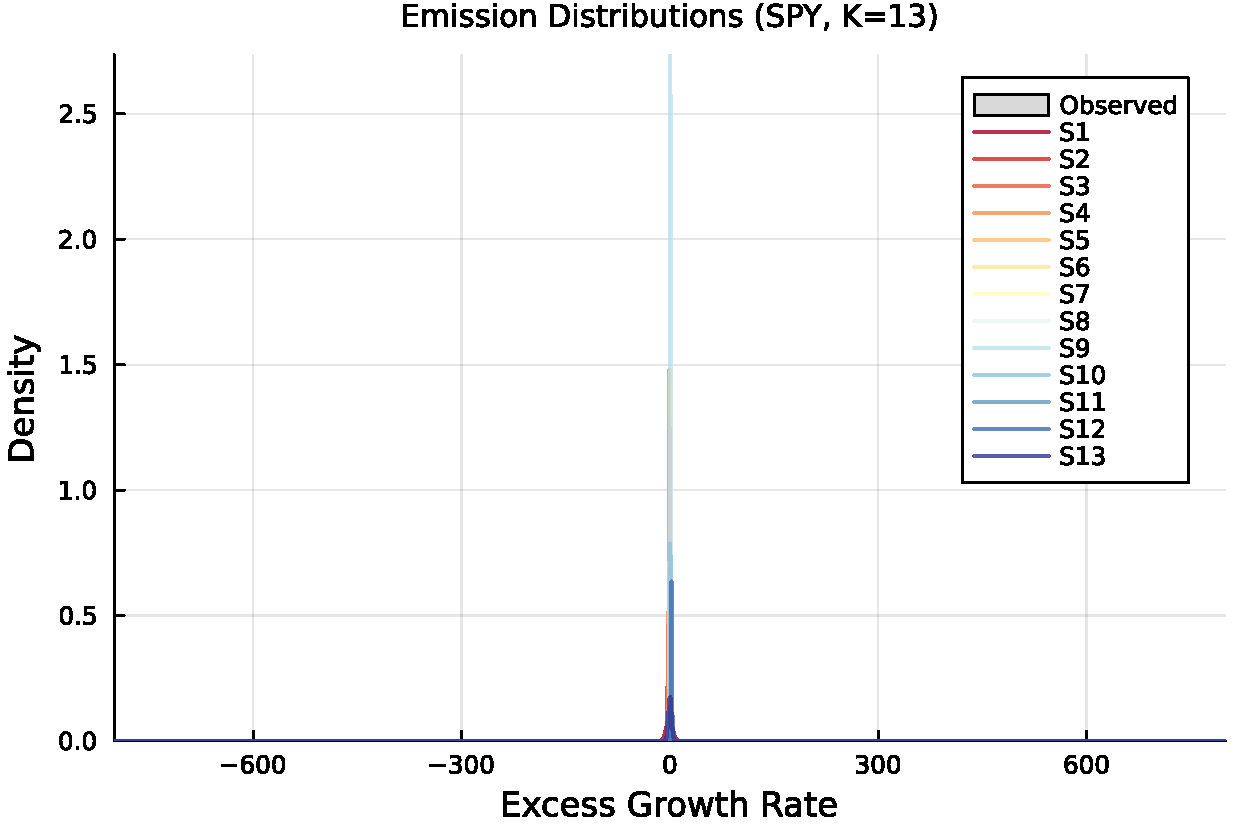
\includegraphics[width=\textwidth]{sections/figs/Fig-Emission-PDFs-K13.pdf}
    \caption{$K = 13$}
\end{subfigure}
\caption{Learned Gaussian emission distributions across state resolutions. Higher $K$ values produce finer decomposition of the return distribution, with dedicated states capturing tail behavior.}
\label{fig:emissions_all}
\end{figure}

\subsection{ACF Comparison at Optimal Parameters}

Figure~\ref{fig:acf_optimal_all} shows the ACF of $|G_t|$ at the optimal jump parameters for $K = 3$ and $K = 13$.

\begin{figure}[H]
\centering
\begin{subfigure}[b]{0.48\textwidth}
    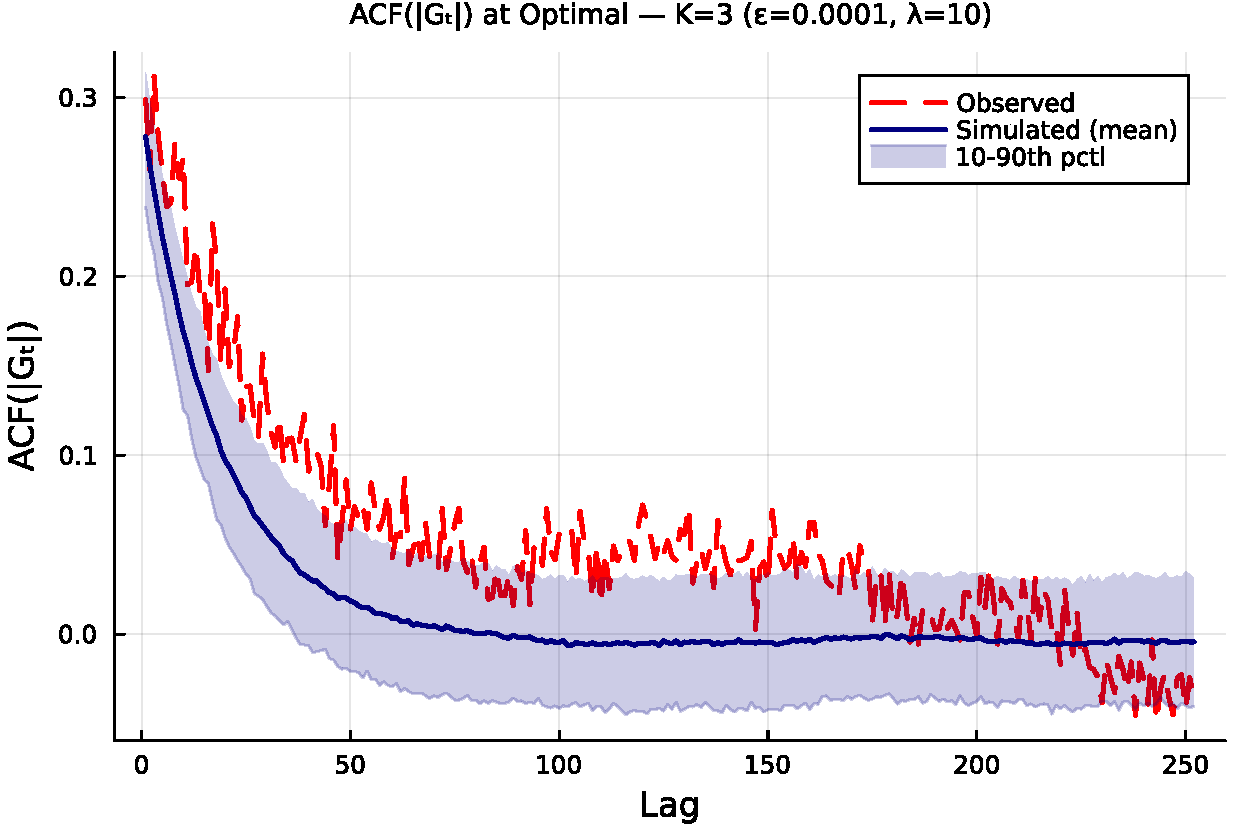
\includegraphics[width=\textwidth]{sections/figs/Fig-ACF-Optimal-K3.pdf}
    \caption{$K = 3$}
\end{subfigure}
\hfill
\begin{subfigure}[b]{0.48\textwidth}
    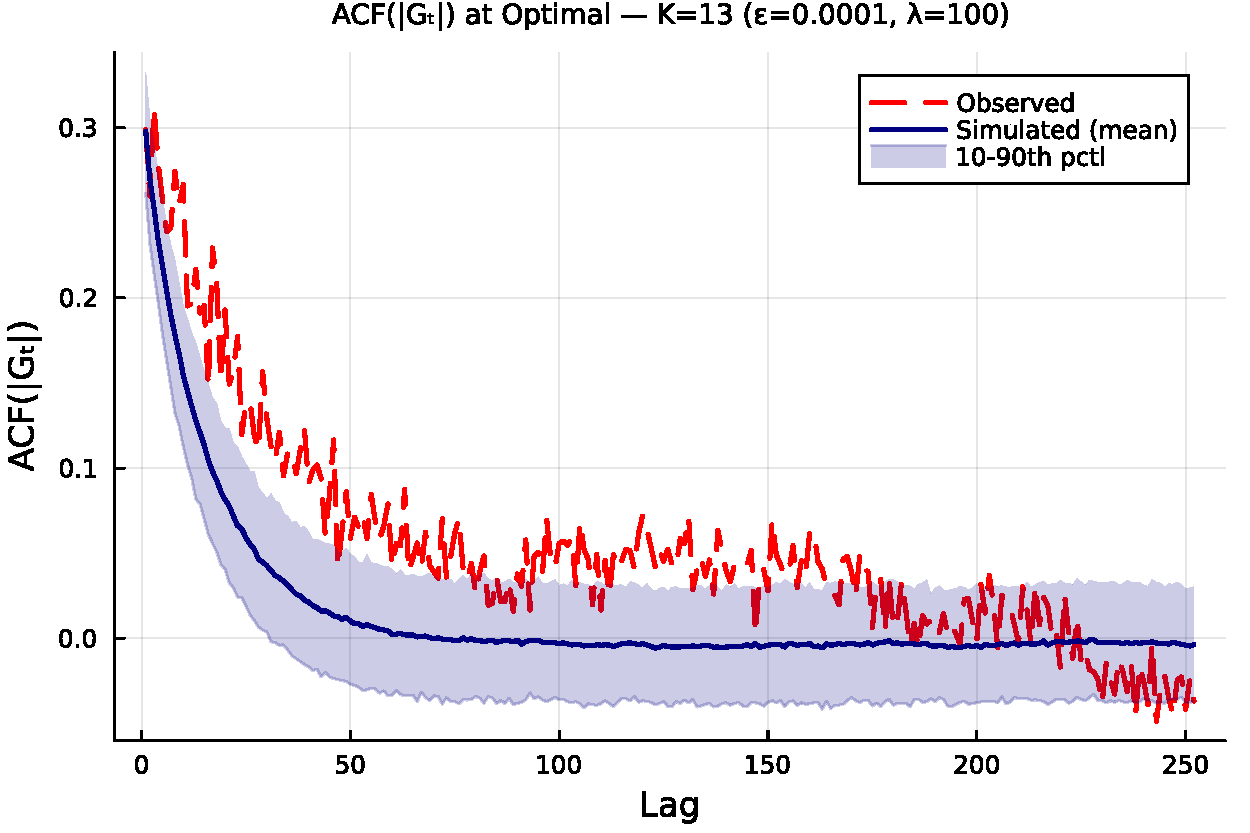
\includegraphics[width=\textwidth]{sections/figs/Fig-ACF-Optimal-K13.pdf}
    \caption{$K = 13$}
\end{subfigure}
\caption{ACF of $|G_t|$ at optimal jump parameters. The simulated 10th--90th percentile envelope (shaded) partially envelopes the observed ACF (red dashed).}
\label{fig:acf_optimal_all}
\end{figure}

\subsection{Stationary Distributions}

\begin{figure}[H]
\centering
\begin{subfigure}[b]{0.48\textwidth}
    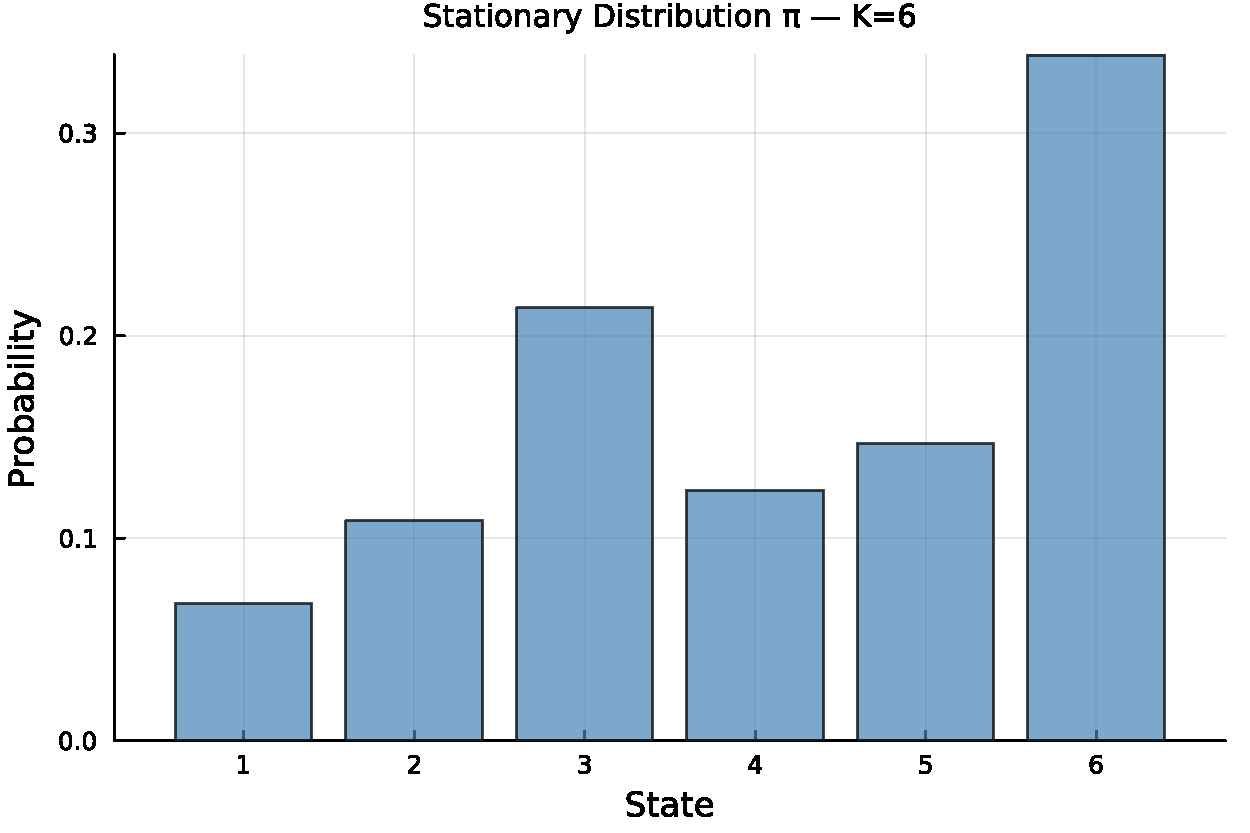
\includegraphics[width=\textwidth]{sections/figs/Fig-Stationary-Distribution-K6.pdf}
    \caption{$K = 6$}
\end{subfigure}
\hfill
\begin{subfigure}[b]{0.48\textwidth}
    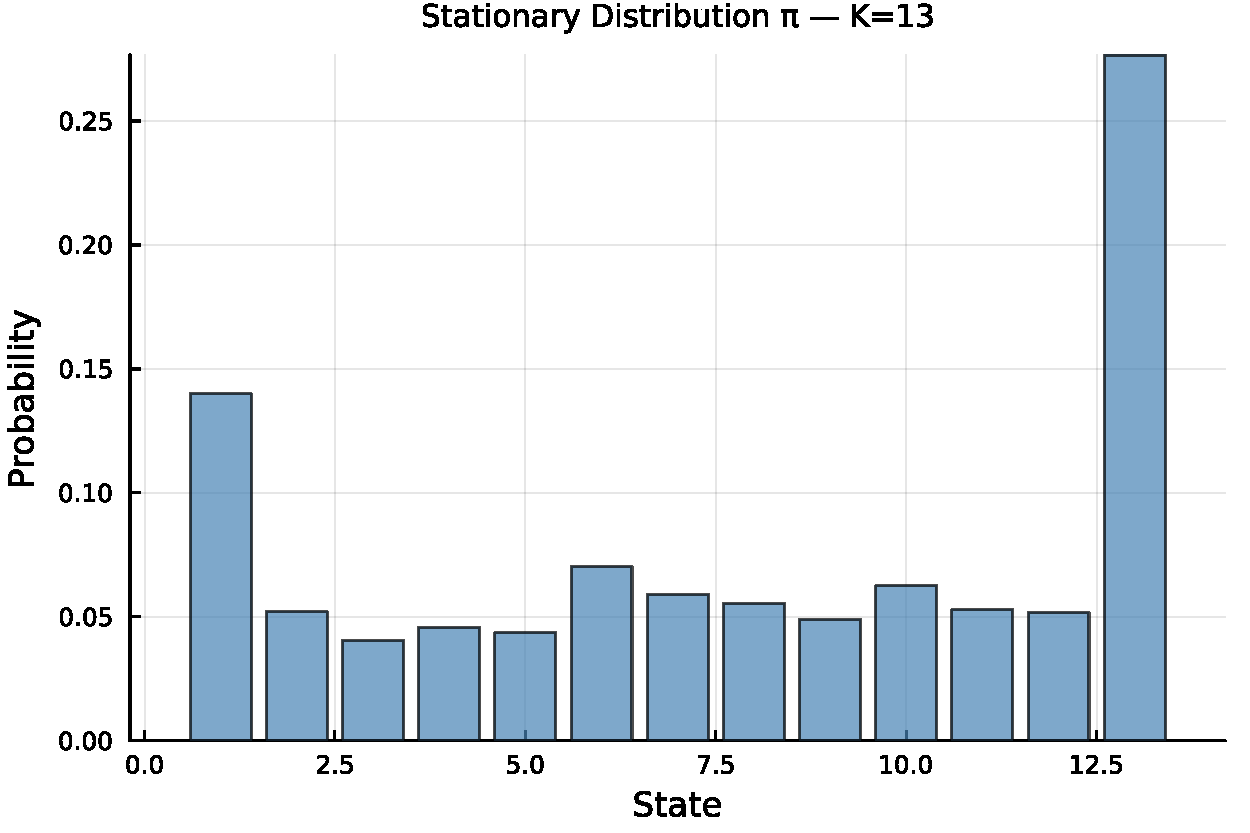
\includegraphics[width=\textwidth]{sections/figs/Fig-Stationary-Distribution-K13.pdf}
    \caption{$K = 13$}
\end{subfigure}
\caption{Stationary distributions $\bar{\pi}$ for $K = 6$ and $K = 13$. Central states receive the highest stationary probability, consistent with the concentration of returns near zero.}
\label{fig:stationary_all}
\end{figure}

\subsection{Residence Times}

\begin{figure}[H]
\centering
\begin{subfigure}[b]{0.48\textwidth}
    
\includegraphics[width=\textwidth]{sections/figs/Fig-Residence-Times-K6.pdf}
    \caption{$K = 6$}
\end{subfigure}
\hfill
\begin{subfigure}[b]{0.48\textwidth}
    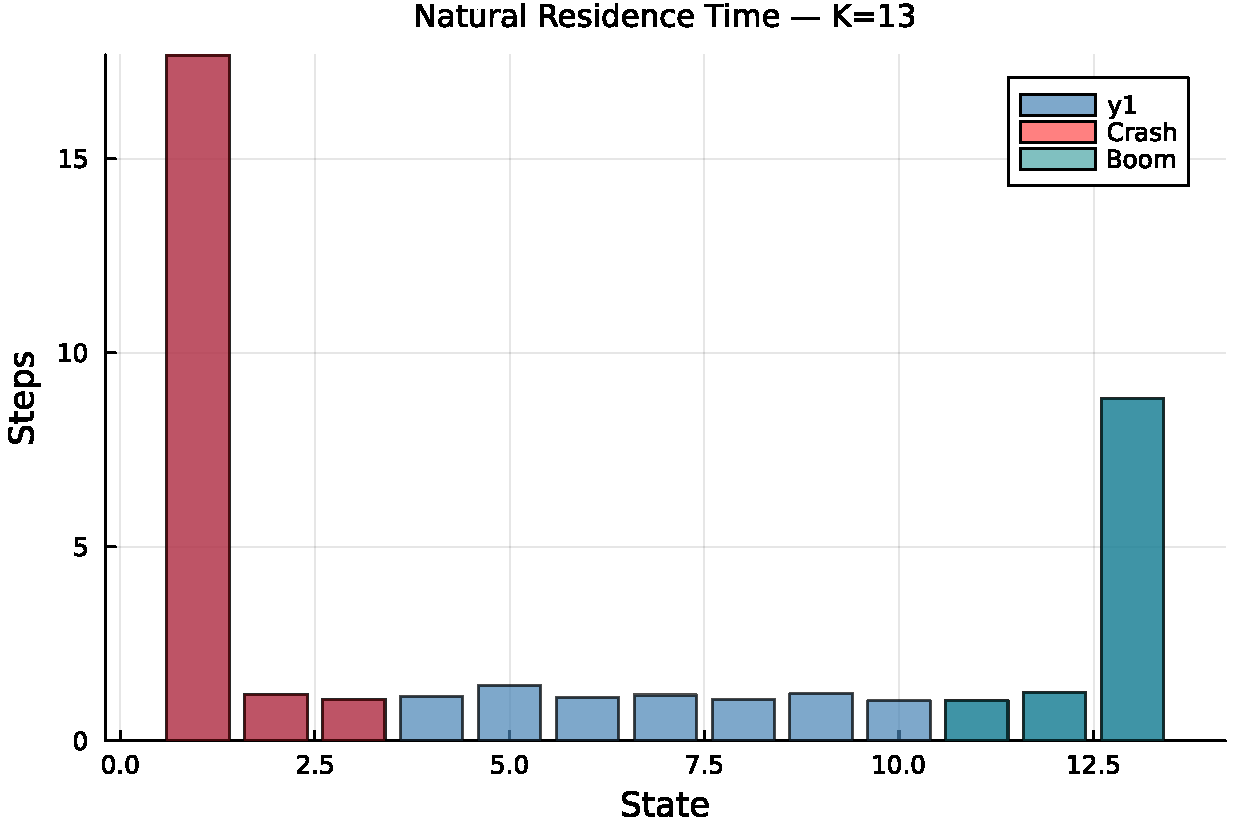
\includegraphics[width=\textwidth]{sections/figs/Fig-Residence-Times-K13.pdf}
    \caption{$K = 13$}
\end{subfigure}
\caption{Natural residence times $1/(1 - T_{kk})$ per state. Under pure Markov dynamics, all states---including crash (red) and boom (teal) tails---exit within 1--2 steps, motivating the jump-duration extension.}
\label{fig:residence_all}
\end{figure}
